\chap{Un robot de compagnie}\label{ch.pet}

Un \emph{robot autonome} adopte un comportement spécifique en fonction de la situation dans laquelle il se trouve.
Il arrive à réagir grâce au \textit{feedback}, littéralement <<\,l'information en retour\,>> en anglais.
Il faut donc que le robot puisse «\,voir\,» le monde qui l'entoure pour pouvoir y réagir.

\sect{Thymio vous obéit}

Nous allons programmer Thymio pour qu'il vous obéisse:
le robot restera sur place sans bouger, mais quand il détectera votre main devant lui, il bougera dans sa direction.

{\raggedleft \hfill Programme: \bu{obeys.aesl}}

Thymio a cinq capteurs de proximité horizontaux à l'avant et deux à l'arrière.
Ils sont similaires à ceux qui se trouve sous Thymio et que nous avons utilisés au \cref{ch.moving}.
Avancez votre main en direction des capteurs à l'avant de Thymio et vous verrez une lumière rouge apparaître à côté du capteur qui vous aura détecté, comme sur la \cref{fig.detect}.

\begin{figure}
\begin{center}
\gr{detect}{.5}
\caption{L'avant de Thymio. Deux doigts sont détectés par les capteurs avant.}\label{fig.detect}
\end{center}
\end{figure}

Le bloc \blksm{event-prox} sert à détecter si quelque chose est proche d'un des capteurs horizontaux avants et arrières de Thymio.
Dans les deux cas, un événement est déclenché.
Les petits carrés gris (cinq sur l'avant et deux sur l'arrière) sont utilisés comme pour les capteurs situés sous Thymio.
En cliquant dessus, ils passent de gris à blanc, à noir et à nouveau à gris.
Les significations des couleurs sont :

\begin{itemize}
\item \textbf{Gris} : Le capteur n'est pas utilisé.
\item \textbf{Blanc} : L'action associée est déclenchée s'il y a beaucoup de lumière réfléchie.
\label{p.proximity-colors2}
Le carré blanc a un bord rouge pour vous rappeler que l'événement sera déclenché lorsque les lumières à côtés des capteurs seront elles-mêmes allumées.
\item \textbf{Noir} : L'action associée est déclenchée s'il y a peu de lumière réfléchie.
\end{itemize}

Si vous souhaitez qu'un événement se produise quand un objet est proche d'un capteur, utilisez les carrés blancs car l'objet 
réfléchira beacoup de lumière.
Si vous souhaitez au contraire qu'un événement se produise
quand aucun objet ne se trouve à proximité d'un capteur,
utilisez un carré noir car peu de lumière sera réfléchie.

Pour construire le comportement, il nous faut deux paires événement-actions, (\cref{fig.follow-hand}).
Dans ce programme, vous voyez que dans la première paire, le carré central est noir et l'action associée est que les moteurs sont arrêtés.
Ainsi, lorsque le robot ne voit rien, il ne bougera pas ; et s'il bougeait, il s'arrêtera.
Dans la deuxième paire, le carré central est rouge et les \textit{sliders} du bloc action moteurs sont glissés vers le haut.
Ainsi, lorsque vous amenez votre main près de l'avant du robot, un événement se produit qui fait tourner les deux moteurs assez vite et fait avancer le robot en avant.


\begin{figure}
\begin{floatrow}
	\ffigbox
	{\caption{Thymio avance vers votre main}\label{fig.follow-hand}}
	{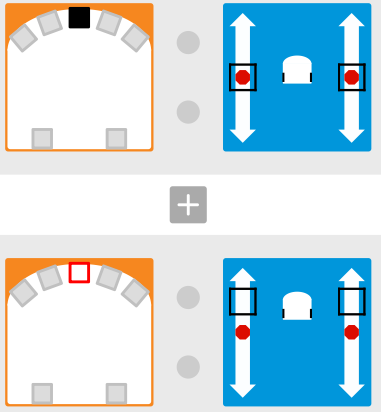
\includegraphics[width=.4\textwidth]{likes-forward}}
	\ffigbox
	{\caption{Un bulldozer à chenilles}\label{fig.bull}}
	{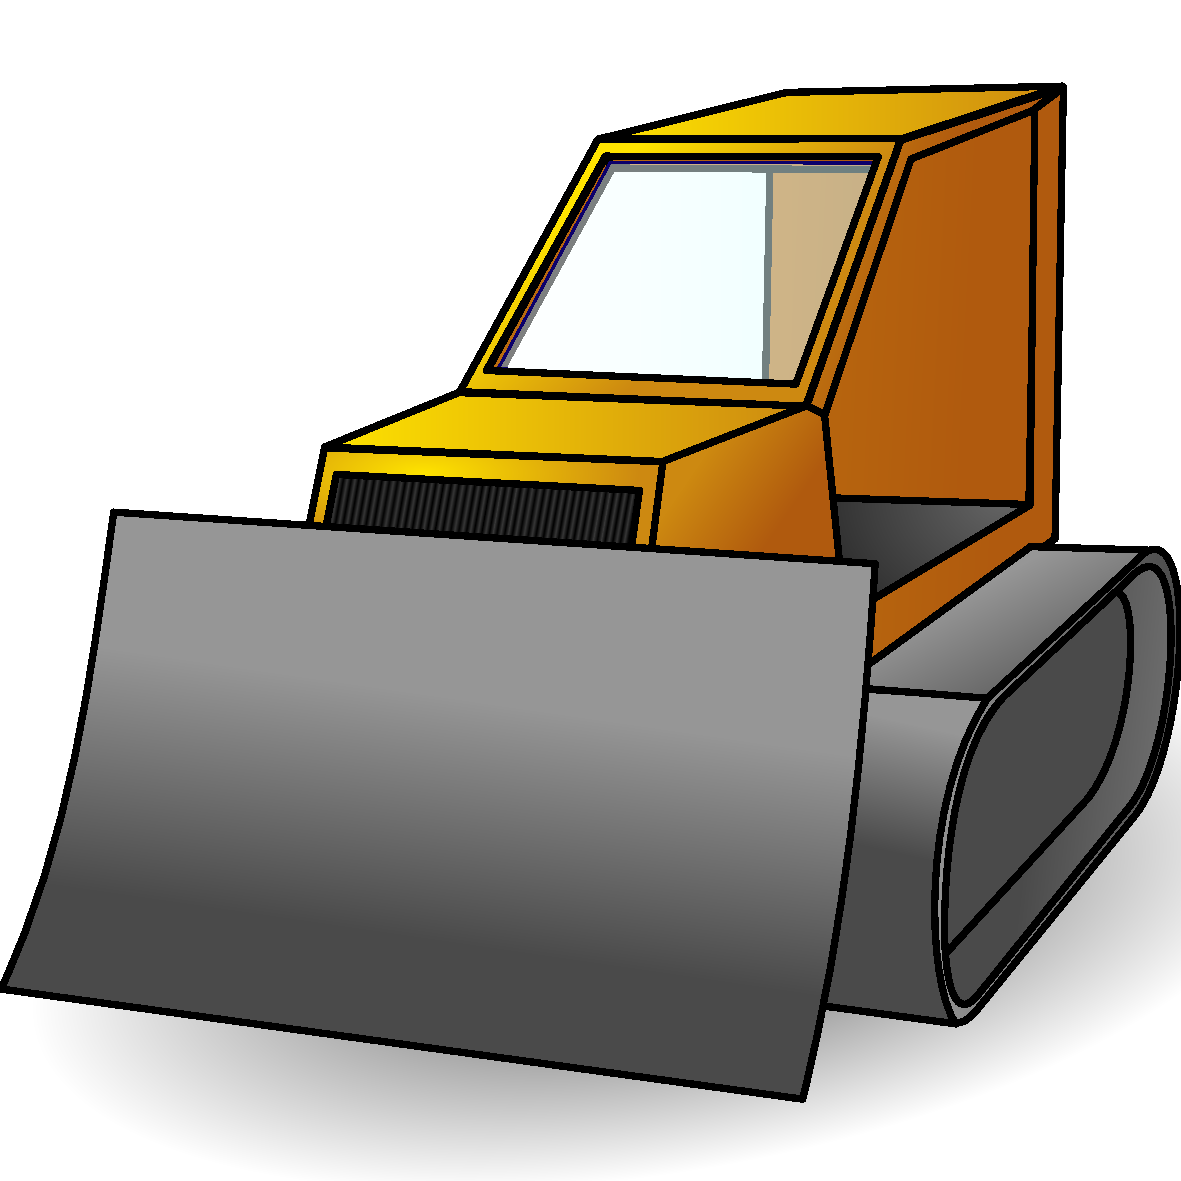
\includegraphics[width=.35\textwidth]{bulldozer}}
\end{floatrow}
\end{figure}

\sect{Faire tourner Thymio}

Thymio n'a pas un volant comme une voiture ou un guidon comme un vélo.
Comment tourne-t-il donc ? 
Pour tourner, le robot utilise une \emph{direction différentielle}, ou \emph{differential drive} en anglais, qui est  utilisée par de nombreux véhicules à chenilles comme le bulldozer sur la \cref{fig.bull}.
À la place de tourner un guidon dans la direction désirée, les chenilles ou roues gauches et droites sont commandées par des moteurs individuels à des vitesses \emph{différentes}.
Si la roue droite tourne plus vite que la roue gauche, alors le véhicule tournera à gauche, tandis que si sa roue gauche tourne plus vite que sa roue droite, il tournera à droite.

La direction différentielle pour le Thymio est réalisée 
en réglant les différents \textit{sliders} d'un bloc action moteurs à des endroits différents, de sorte que les roues de Thymio ne tourneront pas à la même vitesse, ce qui fera tourner le robot.
Plus la différence de vitesse est élevée, plus le virage sera serré.
Pour arriver à une grande différence de vitesses, vous pouvez faire tourner une roue en avant et l'autre en arrière.
En fait, pour tourner sur lui-même, il suffit à Thymio de faire tourner ses deux roues à la même vitesse mais dans des sens opposés !
Par exemple, dans ce bloc action moteurs \blksm{differential}, le \textit{slider} gauche indique une grande vitesse en arrière, alors que le \textit{slider} droite indique une grande vitesse en avant.
Le résultat est que le robot tournera sur lui-même en direction de la gauche, comme indiqué par l'image du robot.

Testez la paire événement-action suivante: \blkc{turning}

Si vous chargez ensuite ce programme et appuyez sur le bouton central, Thymio tournera sur lui-même. Vous pouvez toujours l'arrêter en appuyant sur \blksm{stop}.
Vous pouvez maintenant changer les \textit{sliders} et réessayer.

\trickbox{L'icône du Thymio au centre du bloc action moteurs s'anime dès que vous réglez les \textit{sliders} pour vous donner une idée du mouvement de Thymio!
Lorsque l'animation s'arrête, l'image donne la direction dans laquelle le robot se déplacera quand il exécutera ce bloc action.}

\sect{Thymio vous aime}

Un vrai animal de compagnie ne se contente pas de s'approcher ou de s'éloigner de vous, il vous suit un peu partout! 
Pour que Thymio puisse vous suivre le plus fidèlement possible, il faudra ajouter deux paires événement-actions au programme précédant.
Si Thymio vous détecte avec son capteur tout à droite, il doit tourner à droite et s'il vous détecte avec son capteur tout à gauche, il doit tourner à gauche.

{\raggedleft \hfill Programme: \bu{likes.aesl}}

Une façon de faire est illustrée sur la \cref{fig.likes}.
Vous pouvez essayer différentes vitesses, le faire tourner sur lui-même ou non, afin de trouver le meilleur comportement !

\begin{figure}
	\subfigure[Thymio s'oriente face à vous]{
		\label{fig.likes}
		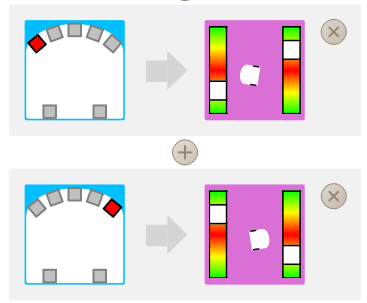
\includegraphics[width=.4\textwidth]{likes-turns}
	}
	\hfill
	\subfigure[Thymio vous évite]{
		\label{fig.hates}
		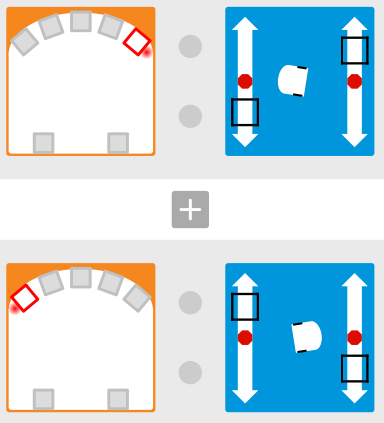
\includegraphics[width=.4\textwidth]{hates}
	}
        \caption{Programmes pour le robot de compagnie}\label{fig.likes-hates}
\end{figure}

\exercisebox{\thechapter.1}{
Modifiez le comportement du robot de compagnie pour qu'il bouge en avant quand le programme est exécuté et qu'il s'arrête lorsqu'il détecte le bord de la table (ou une bande de ruban adhésif noir).}

\exercisebox{\thechapter.2}{
Qu'arrive-t-il si vous changez l'ordre des paires événement-actions utilisées dans l'exercice précédent ?
}


\sect{Thymio ne vous aime pas}

Parfois, même le plus fidèle animal de compagnie n'a pas envie de vous suivre. 
Écrivez un programme qui génère ce comportement.

{\raggedleft \hfill Programme: \bu{does-not-like.aesl}}

Ouvrez le programme du Thymio qui vous aime et inversez l'association des événements avec les actions.
Détecter un objet avec le capteur gauche fait tourner le robot à droite, et détecter un objet avec le capteur droite fait tourner le robot à gauche (\cref{fig.hates}).

% \begin{figure}[h]
%     \centering
%     \subfigure[S'il vous détecte devant lui, il recule]{ \label{fig.recule} 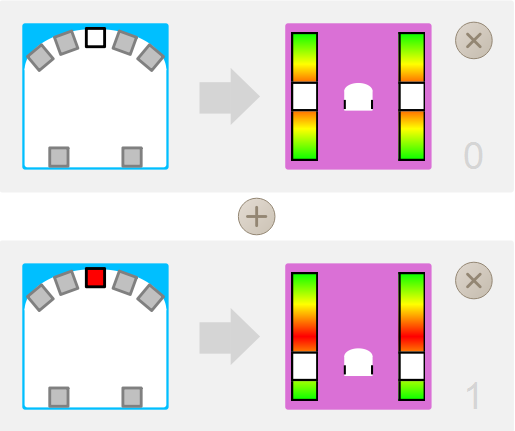
\includegraphics[width = 0.35\textwidth]{hates2}}
%     \hspace{1cm}
%     \subfigure[S'il vous détecte sur les côtés, il vous évite]{ \label{fig.evite} 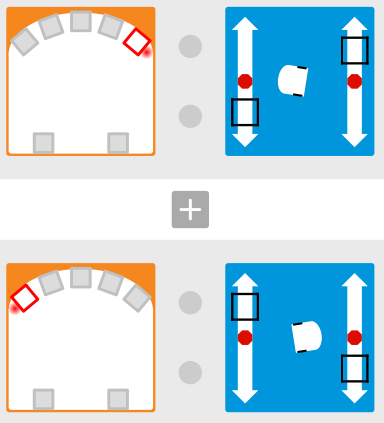
\includegraphics[width = 0.35\textwidth]{hates}}
%     \caption{Thymio vous évite et vous fuit}
%     \label{fig.recule-evite}
% \end{figure}

\exercisebox{\thechapter.3}
{
Les capteurs horizontaux avant sont numérotés 0, 1, 2, 3, 4 de gauche à droite.
Les capteurs arrière sont numérotés 5 pour le gauche et 6 pour le droite.
À la place d'utiliser les capteurs 0 et 4 comme jusqu'à maintenant:
\begin{itemize}[noitemsep,nosep,leftmargin=*]
\item Utilisez le capteur 1 pour tourner le robot vers la gauche et le 3 pour tourner vers la droite.
\item Utilisez à la fois les capteurs 0 et 1 pour tourner le robot à gauche et à la fois les capteurs 3 et 4 pour tourner le robot à droite.
\item Ajouter une paire événement-actions pour les capteurs arrières 5 et 6.
\end{itemize}
}

\bigskip

\trickbox{L'\cref{a.tech} montre comment régler les \textit{sliders} à des vitesses précises.}

\bigskip

\informationbox{Les capteurs en mode avancé}{
En mode avancé (\cref{ch.time}), il existe un quatrième bloc
qui permet de spécifier quand les capteurs génèrent
des événements, en plus des modes gris, blanc et noir. Référez-vous à l'\cref{a.tech}.}
